\documentclass{ximera}
%\usepackage{todonotes}

\usepackage{tkz-euclide}
\usetikzlibrary{backgrounds} %% for boxes around graphs
\usetikzlibrary{shapes,positioning}  %% Clouds and stars
\usetkzobj{all}
\usepackage[makeroom]{cancel} %% for strike outs
%\usepackage{mathtools} %% for pretty underbrace % Breaks Ximera
\usepackage{multicol}


\newcommand{\RR}{\mathbb R}
\renewcommand{\d}{\,d}
\newcommand{\dd}[2][]{\frac{d #1}{d #2}}
\renewcommand{\l}{\ell}
\newcommand{\ddx}{\frac{d}{dx}}
\newcommand{\zeroOverZero}{$\boldsymbol{\tfrac{0}{0}}$}
\newcommand{\numOverZero}{$\boldsymbol{\tfrac{\#}{0}}$}
\newcommand{\dfn}{\textbf}
\newcommand{\eval}[1]{\bigg[ #1 \bigg]}
\renewcommand{\epsilon}{\varepsilon}
\renewcommand{\iff}{\Leftrightarrow}

\DeclareMathOperator{\arccot}{arccot}
\DeclareMathOperator{\arcsec}{arcsec}
\DeclareMathOperator{\arccsc}{arccsc}


\colorlet{textColor}{black} 
\colorlet{background}{white}
\colorlet{penColor}{blue!50!black} % Color of a curve in a plot
\colorlet{penColor2}{red!50!black}% Color of a curve in a plot
\colorlet{penColor3}{red!50!blue} % Color of a curve in a plot
\colorlet{penColor4}{green!50!black} % Color of a curve in a plot
\colorlet{penColor5}{orange!80!black} % Color of a curve in a plot
                                      \colorlet{fill1}{blue!50!black!20} % Color of fill in a plot
\colorlet{fill2}{blue!10} % Color of fill in a plot
\colorlet{fillp}{fill1} % Color of positive area
\colorlet{filln}{red!50!black!20} % Color of negative area
\colorlet{gridColor}{gray!50} % Color of grid in a plot

\pgfmathdeclarefunction{gauss}{2}{% gives gaussian
  \pgfmathparse{1/(#2*sqrt(2*pi))*exp(-((x-#1)^2)/(2*#2^2))}%
}



\newcommand{\fullwidth}{}
\newcommand{\normalwidth}{}



%% makes a snazzy t-chart for evaluating functions
\newenvironment{tchart}{\rowcolors{2}{}{background!90!textColor}\array}{\endarray}

%%This is to help with formatting on future title pages.
\newenvironment{sectionOutcomes}{}{} 

\author{Emma Smith Zbarsky}
\license{Creative Commons Attribution 3.0 Unported}
\acknowledgement{https://quadbase.org/questions/q14590v1}
\begin{document}

\begin{exercise}

As you get older, you are likely to move off-campus into an apartment.
You have decided to rent an apartment where the entry hall has the
following geometry:

\begin{image}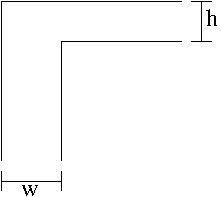
\includegraphics[width=.5\textwidth]{corner.jpg}\end{image}

 If $h=3$ ft and $w=4$ ft, what is
the maximum length of a straight, rigid object you can carry around the
corner into your apartment? Assume you carry it horizontally to the
floor. Give your answer to the nearest hundredth of a foot.

`'Hint: Consider working with angles.''


\begin{hint}
This is an optimization problem. You should write down a formula that
computes the distance from the left hand wall to the top wall passing by
the inside corner, then find the extrema.
\end{hint}


\begin{hint}
First, label your diagram: \{img:corner-labeled\_1.jpg\} Then, write
down the equation describing the length of $L = L_1+L_2$. Because
\[\cos(\theta) = \frac{w}{L_1}\] and \[\sin(\theta) = \frac{h}{L_2}\] we
see that
\[L = L_1+L_2 = \frac{w}{\cos(\theta)}+\frac{h}{\sin(\theta)} = 4\sec(\theta)+3\csc(\theta).\]
Calculating the derivative, we have:
\begin{align*} L' &= 4\sec(\theta)\tan(\theta)-3\csc(\theta) \cot(\theta) = 0 \\
3\csc(\theta)\cot(\theta) &= 4\sec(\theta)\tan(\theta) \\
\frac{3\cos(\theta)}{\sin^2(\theta)} &= \frac{4\sin(\theta)}{\cos^2(\theta)} \\
\frac{3}{4} &= \frac{\sin^3(\theta)}{\cos^3(\theta)} = \tan^3(\theta) \\
\theta &= \arctan\left(\left(\frac{3}{4}\right)^{1/3}\right) \\
& \simeq   0.737524
\end{align*} This gives us a length of
\[L \simeq 4\sec(0.737524)+3\csc(0.737524) = 9.86566,\] or about 9.87
feet or 9 feet 10 3/4 inches.
\end{hint}


\begin{multipleChoice}
\choice{9.89 feet}
\choice{9.85 feet}
\choice{9.93 feet}
\choice[correct]{9.87 feet}
\choice{9.91 feet}
\end{multipleChoice}

\end{exercise}
\end{document}
